
\documentclass{sig-alternate-issta}
\usepackage{multirow}
\usepackage{fancyheadings}
\usepackage{algorithmic}
\usepackage{amssymb}
\usepackage{amsmath}
\usepackage{xspace}
\usepackage{pslatex}
\usepackage{microtype}
\usepackage{subfigure}
\usepackage{indentfirst}
\usepackage{listings, algorithm, algorithmic, graphicx, listing}
\usepackage{relsize}
\usepackage{fancyvrb}

\usepackage{balance}

%\usepackage{todonotes}
%\usepackage{times}
\usepackage{graphicx}
\usepackage{epsf}
\usepackage{verbatim}
%\usepackage{psfig}
\usepackage{cite}
\usepackage{url}
\usepackage{color}
\usepackage{alltt}

\newcommand{\StateProjection}{static analysis}
\newcommand{\CurAspectJSubjectCount}{12}

\newcommand{\Add}{\CodeIn{add}}
\newcommand{\AVTree}{\CodeIn{AVTree}}
\newcommand{\Assignment}[3]{$\langle$ \Object{#1}, \Object{#2}, \Object{#3} $\rangle$}
\newcommand{\BinaryTreeRemove}{\CodeIn{BinaryTree\_remove}}
\newcommand{\BinaryTree}{\CodeIn{BinaryTree}}
\newcommand{\Caption}{\caption}
\newcommand{\Char}[1]{`#1'}
\newcommand{\CheckRep}{\CodeIn{checkRep}}
\newcommand{\ClassC}{\CodeIn{C}}
\newcommand{\CodeIn}[1]{{\small\texttt{#1}}}
\newcommand{\CodeOutSize}{\scriptsize}
\newcommand{\Comment}[1]{}
\newcommand{\Ensures}{\CodeIn{ensures}}
\newcommand{\ExtractMax}{\CodeIn{extractMax}}
\newcommand{\FAL}{field-ordering}
\newcommand{\FALs}{field-orderings}
\newcommand{\Fact}{observation}
\newcommand{\Get}{\CodeIn{get}}
\newcommand{\HashSet}{\CodeIn{HashSet}}
\newcommand{\HeapArray}{\CodeIn{HeapArray}}
\newcommand{\Intro}[1]{\emph{#1}}
\newcommand{\Invariant}{\CodeIn{invariant}}
\newcommand{\JUC}{\CodeIn{java.\-util.\-Collections}}
\newcommand{\JUS}{\CodeIn{java.\-util.\-Set}}
\newcommand{\JUTM}{\CodeIn{java.\-util.\-TreeMap}}
\newcommand{\JUTS}{\CodeIn{java.\-util.\-TreeSet}}
\newcommand{\JUV}{\CodeIn{java.\-util.\-Vector}}
\newcommand{\JMLPlusJUnit}{JML+JUnit}
\newcommand{\Korat}{Korat}
\newcommand{\Left}{\CodeIn{left}}
\newcommand{\Lookup}{\CodeIn{lookup}}
\newcommand{\MethM}{\CodeIn{m}}
\newcommand{\Node}[1]{\CodeIn{N}$_#1$}
\newcommand{\Null}{\CodeIn{null}}
\newcommand{\Object}[1]{\CodeIn{o}\ensuremath{_#1}}
\newcommand{\PostM}{\MethM$_{post}$}
\newcommand{\PreM}{\MethM$_{pre}$}
\newcommand{\Put}{\CodeIn{put}}
\newcommand{\Remove}{\CodeIn{remove}}
\newcommand{\RepOk}{\CodeIn{repOk}}
\newcommand{\Requires}{\CodeIn{requires}}
\newcommand{\Reverse}{\CodeIn{reverse}}
\newcommand{\Right}{\CodeIn{right}}
\newcommand{\Root}{\CodeIn{root}}
\newcommand{\Set}{\CodeIn{set}}
\newcommand{\State}[1]{2^{#1}}
\newcommand{\TestEra}{TestEra}
\newcommand{\TreeMap}{\CodeIn{TreeMap}}

\newenvironment{CodeOut}{\begin{scriptsize}}{\end{scriptsize}}
\newenvironment{SmallOut}{\begin{small}}{\end{small}}

\newcommand{\pairwiseEquals}{PairwiseEquals}
\newcommand{\monitorEquals}{MonitorEquals}
%\newcommand{\monitorWField}{WholeStateW}
\newcommand{\traverseField}{WholeState}
\newcommand{\monitorSMSeq}{ModifyingSeq}
\newcommand{\monitorSeq}{WholeSeq}

\newcommand{\IntStack}{\CodeIn{IntStack}}
\newcommand{\UBStack}{\CodeIn{UBStack}}
\newcommand{\BSet}{\CodeIn{BSet}}
\newcommand{\BBag}{\CodeIn{BBag}}
\newcommand{\ShoppingCart}{\CodeIn{ShoppingCart}}
\newcommand{\BankAccount}{\CodeIn{BankAccount}}
\newcommand{\BinarySearchTree}{\CodeIn{BinarySearchTree}}
\newcommand{\LinkedList}{\CodeIn{LinkedList}}

\newcommand{\Book}{\CodeIn{Book}}
\newcommand{\Library}{\CodeIn{Library}}

\newcommand{\Jtest}{Jtest}
\newcommand{\JCrasher}{JCrasher}
\newcommand{\Daikon}{Daikon}
\newcommand{\JUnit}{JUnit}

\newcommand{\trie}{trie}

\newcommand{\Perl}{Perl}


\newcommand{\SubjectCount}{11}
\newcommand{\DSSubjectCount}{two}

\newcommand{\Equals}{\CodeIn{equals}}
\newcommand{\Pairwise}{PairwiseEquals}
\newcommand{\Subgraph}{MonitorEquals}
\newcommand{\Concrete}{WholeState}
\newcommand{\ModSeq}{ModifyingSeq}
\newcommand{\Seq}{WholeSeq}
\newcommand{\Aeq}{equality}

\newcommand{\Meaning}[1]{\ensuremath{[\![}#1\ensuremath{]\!]}}
\newcommand{\Pair}[2]{\ensuremath{\langle #1, #2 \rangle}}
\newcommand{\Triple}[3]{\ensuremath{\langle #1, #2, #3 \rangle}}
\newcommand{\SetSuch}[2]{\ensuremath{\{ #1 | #2 \}}}
%\Comment{
%\newtheorem{definition}{Definition}
%\newtheorem{theorem}[definition]{Theorem}
%}
\newcommand{\Equiv}[2]{\ensuremath{#1 \EquivSTRel{} #2}}
\newcommand{\EquivME}{\Equiv}
\newcommand{\EquivST}{\Equiv}
\newcommand{\EquivSTRel}{\ensuremath{\cong}}
\newcommand{\Redundant}[2]{\ensuremath{#1 \lhd #2}}
\newcommand{\VB}{\ensuremath{\mid}}
\newcommand{\MES}{method-entry state}

\newcommand{\Small}[1]{{\small{#1}}}

\newcommand{\CenterCell}[1]{\multicolumn{1}{c|}{#1}}
\newcommand{\Fix}[1]{{\large\textbf{FIX}}#1{\large\textbf{FIX}}}

\newcommand{\CodeInS}[1]{{\scriptsize\texttt{#1}}}
\newcommand{\CodeInFN}[1]{{\footnotesize\texttt{#1}}}
\newcommand{\CodeOutFN}{\footnotesize}

\newcommand{\SmallSpace}{\vspace*{-1.4ex}}
\newcommand{\Item}{\SmallSpace\item}
\newenvironment{Itemize}{\begin{itemize}}{\end{itemize}\SmallSpace}
\newenvironment{Enumerate}{\begin{enumerate}}{\end{enumerate}\SmallSpace}

% Permit line breaking
\newcommand{\dependenceaware}{de\-pend\-ence-aware}

%\newtheorem{definition}{Definition}
%\newtheorem{theorem}[definition]{Theorem}

%\newcommand{\Item}{\vspace*{-0.5ex}\item\vspace*{-0.5ex}}
%\newenvironment{Itemize}{\begin{itemize}\vspace*{-1ex}}{\end{itemize}\vspace*{-1ex}}
%\newenvironment{Enumerate}{\begin{enumerate}\vspace*{-1ex}}{\end{enumerate}\vspace*{-1ex}}
\newenvironment{Definition}{\begin{definition}\vspace*{-1.5ex}}{\end{definition}\vspace*{-1.5ex}}

% Local Variables:
% mode:latex
% tex-main-file:"ase04.tex"
% End:


%% Comment out one of these two definitions.
% \newcommand{\todo}[1]{\relax}
\newcommand{\todo}[1]{{\color{red}\bfseries [[#1]]}}

% Add line between figure and text
\makeatletter
\def\topfigrule{\kern3\p@ \hrule \kern -3.4\p@} % the \hrule is .4pt high
\def\botfigrule{\kern-3\p@ \hrule \kern 2.6\p@} % the \hrule is .4pt high
\def\dblfigrule{\kern3\p@ \hrule \kern -3.4\p@} % the \hrule is .4pt high
\makeatother
% If there is a line, you can get away with reducing the separation between
% figures and text.  Don't do this without the line, though.
\addtolength{\textfloatsep}{-.5\textfloatsep}
\addtolength{\dbltextfloatsep}{-.5\dbltextfloatsep}
\addtolength{\floatsep}{-.5\floatsep}
\addtolength{\dblfloatsep}{-.5\dblfloatsep}

% At least 80% of every float page must be taken up by
% floats; there will be no page with more than 20% white space.
\def\topfraction{.8}
\def\dbltopfraction{\topfraction}
\def\floatpagefraction{\topfraction}     % default .5
\def\dblfloatpagefraction{\topfraction}  % default .5
\def\textfraction{.2}

% Left and right curly braces in tt font
\newcommand{\ttlcb}{\texttt{\char "7B}}
\newcommand{\ttrcb}{\texttt{\char "7D}}

% \|name| or \mathid{name} denotes identifiers and slots in formulas
\def\|#1|{\mathid{#1}}
\newcommand{\mathid}[1]{\ensuremath{\mathit{#1}}}
% \<name> or \codeid{name} denotes computer code identifiers
\def\<#1>{\codeid{#1}}
\newcommand{\codeid}[1]{\ifmmode{\mbox{\ttfamily{#1}}}\else{\ttfamily #1}\fi}


\newcommand{\smallstep}{\relax}
\newcommand{\tinystep}{\relax}

\newcommand{\yes}{Yes\xspace}

\newcommand{\no}{No\xspace}

\newcommand{\prevtool}{ConfDiagnoser\xspace}
\newcommand{\ourtool}{EvolDiagnoser\xspace}
\newcommand{\missing}{$\bullet$ }

\newcommand{\rest}{REST\xspace}

\newcommand{\dtexplain}{DTExplainer\xspace}

\newcommand{\errornum}{XXX\xspace}
\newcommand{\subjnum}{XXX\xspace}

\newcommand{\selnum}{XXX\xspace}
\newcommand{\prionum}{XXX\xspace}
\newcommand{\parnum}{XXX\xspace}

\newcommand{\preitemizespace}{\vspace{-1mm}}

\renewcommand{\captionfont}{\small\bf}



% Reduce indentation in lists.
%\setlength{\leftmargini}{.5\leftmargini}

%% Bring items closer together in list environments
%% This doesn't work with an optional argument to the list environment.
% Prevent infinite loops
\let\Itemize =\itemize    
\let\Enumerate =\enumerate
\let\Description =\description
% Zero the vertical spacing parameters
\def\Nospacing{\itemsep=0pt\topsep=0pt\partopsep=0pt\parskip=0pt\parsep=0pt}
% Redefine the environments in terms of the original values
\renewenvironment{itemize}{\Itemize\Nospacing}{\endlist}
\renewenvironment{enumerate}{\Enumerate\Nospacing}{\endlist}
\renewenvironment{description}{\Description\Nospacing}{\endlist}

\hyphenation{Wohl-stadt-er}

\begin{document}

\clubpenalty = 10000
\widowpenalty = 10000
\displaywidowpenalty = 10000

\title{When Tests Collide: Evaluating and Coping with\\ the Impact of Test Dependence}
\numberofauthors{1}

\author{
\alignauthor Wing Lam \quad Sai Zhang \quad Michael D. Ernst\\
       \affaddr{Department of Computer Science \& Engineering}\\
       \affaddr{University of Washington}\\
       \email{\{winglam, szhang, mernst\}@cs.washington.edu}
}


\maketitle
\thispagestyle{empty}
\pagestyle{empty}

\begin{abstract}

In a test suite, all the test cases should be independent:  no test
should affect any other test's result, and running the tests in any order
should produce the same test results.
Techniques such as test %selection and
prioritization generally assume that the tests in a suite are independent.
%but they do not justify that assumption.
Test dependence is a little-studied phenomenon.
This paper presents five results related to test dependence.

First, we characterize the test dependence that arises in practice.
We studied \dtnum real-world dependent tests from \repnum
issue tracking systems.
Our study
%  identifies common characteristics of dependent tests.  It 
shows that test dependence can be hard for programmers to identify.
It also shows that test dependence can cause
non-trivial consequences, such as masking
program faults and leading to spurious bug reports.

Second, we formally define test dependence in terms of
test suites as ordered sequences of tests along with explicit
environments in which these tests are executed.
We formulate the problem
of detecting dependent tests and prove that a useful special
case is NP-complete. 

Third, guided by the study of real-world dependent tests, we
propose and compare four algorithms to detect
dependent tests in a test suite. 

Fourth, we applied our dependent test detection algorithms
to \subjnum real-world programs and found
dependent tests 
in each human-written
and automatically-generated test suite.

Fifth, we empirically assessed the impact of
dependent tests on five test prioritization techniques
and found that dependent tests affect the output 
of all five techniques; that is, the reordered suite 
fails even though the original suite did not.

%the follwoing claim might be too strong
%Our tool revealed a large number of previously-unknown dependent tests.
%In our study, on average \todo{xx}\% of the human-written tests are
%dependent and \todo{xx}\% of the automatically-generated tests
%are dependent.

\smallskip
\smallskip


\noindent
\textbf{Categories and Subject Descriptors}:  
D.2.5 [Software Engineering]: Testing and Debugging.
\\
\textbf{General Terms: }
Reliability, Experimentation.
\\
\textbf{Keywords: }
Test dependence, detection algorithms, empirical studies.

\end{abstract}


\label{dummy-label-for-etags}


\section{Introduction}

%\todo{Is ``dependent test'' a term that can be applied to one test in
%  isolation?  Or is a pair of tests dependent on one another if the result
%  of one of them changes if the other one is run first?  The paper doesn't
%  make this clear anywhere in sections 1 and 2, and this leads to some
%  confusion for the reader.}

%Informally, a \emph{dependent test} produces different test
%results when executed in different environments. 
Consider a test suite containing two tests \code{A}
and \code{B}, where running \code{A} and then \code{B} leads
to \code{A} passing, while running \code{B} and then
\code{A} leads to \code{A} failing. We call \code{A}
an \textit{order-dependent} test (in the context of this test suite), since its result depends on
whether it runs after \code{B} or not.



In a test suite, all the test cases should be independent:
no test should affect any other test's result, and
running the tests in any order should produce the same test results.
%Practitioners are well aware of test dependence:  coding
%guidelines~\cite{unit-test-def,Massol:2003} and
%standards~\cite{IEEE:829-1998,IEEE:829-2008} say to avoid or document it,
%and tools support those goals~\cite{junitordering,depunit,testng, easymock, randomjunit}.
%%\todo{Cite a mocking framework}.
%Researchers are also aware of test
%dependence~\cite{Csallner:2004, Steimann:2013, Gray:1994:QGB:191843.191886,Chays:2000:FTD:347324.348954,kapfhammeretal:FSE:2003,Wang:2007:AGC, Samimi:2013:DM}.
%%\todo{Cite research about creating mocks.}
%Nonetheless, much testing research and practice
%assumes test independence;
%this includes techniques for test selection~\cite{harroldetal:OOPSLA:2001,RenCR2006},
%test prioritization~\cite{Elbaum:2000:PTC:347324.348910},
%and test parallelization~\cite{Misailovic:2007}.
%% These are not offected:
%%, test factoring~\cite{Saff:2005}, and test carving~\cite{Elbaum:2006}.
%theoretical results, algorithms, and tools may behave unexpectedly
%in the presence of dependent tests.
%A test suite that contains dependent tests affects the applications
%of these techniques.
%These techniques produce incorrect results if run on a test suite that contains dependent tests. 
%\todo{The claim of the above sentence is too strong, and may irritate readers, given we do not have strong evidence.
%I would tone down it as: dependent tests can
%affect the results of these techniques. Further, the ``correctness''
%of a test selection/prioritization technique is decided by whether
%a test has been selected or not, rather than whether the test should
%maintain the same resutls or not.}
The assumption of test independence 
is important so that testing techniques behave
as designed.
Consider a test prioritization or selection algorithm.  By design, if its
input is a passing test suite, then its output should be a passing test
suite.  If the suite contains an order-dependent test, then prioritization
or selection can introduce test failures, which violates the design
requirement.

Many techniques assume test independence, including test
prioritization~\cite{Elbaum:2000:PTC:347324.348910,
Rummel:2005:TPR:1066677.1067016, Srivastava:2002:EPT:566172.566187, Jiang:2009:ART},
test selection~\cite{harroldetal:OOPSLA:2001, Orso:2004:SRT,
Briand:2009:ART, Zhang:2012:RMT, Nanda:2011:RTP, hsu09may},
test execution~\cite{Kim:2013:OUT, Misailovic:2007},
test factoring~\cite{Saff:2005, Wu:2010:LRV}, test carving~\cite{Elbaum:2006},
and experimental debugging techniques~\cite{Zeller:2002,
Steimann:2013, Zhang:2013:IMF}.
%often implicitly assume no test dependences in
%a test suite. 
%\todo{check the following sentencee, people may ask
%is the above paper list representative enough? be aware.}
%\todo{I think it would be more compelling for this section to only cite
%  papers that do not mention but implicitly assume test independence.  The
%  current writing sounds like you might be cherry-picking:  why this set of
%  papers?  Are the ratios representative?  But if you just give a list (as
%  long as possible) of papers that don't assume it, then that makes the
%  point you want to, and no one will misinterpret the list as trying to be
%  representative.}
However, this critical assumption is
rarely questioned, investigated, or even mentioned:
none of the above papers explicitly mentions the assumption
as a limitation or a threat to validity.
Between 2000 and 2013, 31 papers on test prioritization were
published in the research track of
ICSE, FSE, ISSTA, ASE, and ICST or in
TOSEM and TSE~\cite{alltestprior}.
Of these,
27 papers explicitly or implicitly assumed test independence,
3 papers acknowledged that the potential dependences between tests
may affect\todo{in what way?  be specific} the prioritization output~\cite{Kim:2002:HTP:581339.581357,
Qu:2008:CRT, Rothermel:2004:TSC},
and only 1 paper considered test dependence in the design of
test prioritization algorithms~\cite{10.1109/TSE.2012.26}.

Anecdotally, a number of researchers have told us that they believe test dependence
is not a significant concern in practice.
We wish to investigate the validity of this unverified conventional wisdom,
in order to understand whether test dependence arises in practice, 
the repercussions of dependent tests, and how to 
detect dependent tests.

%is generally ignored.
%Is this acceptable, because test dependence does
%not arise in practice?
%Is it because even when test dependence arises, there are few
%negative repercussions?
%Is it because no one has studied this problem or thought to examine it?
%Is it because the problem is important but is too hard to analyze or understand?

\subsection{Manifest Test Dependence}

%To explore these questions, 
This paper focuses on test
dependence that manifests as a
difference in test result (i.e., passing or failing) as determined by the testing oracle.
We adopt the results of the default
%% True, but a distraction.
% , usually implicit,
order of execution of a test suite as the
expected results; these are the results that a developer sees when running
the suite in the standard way. A test is dependent when there exists a possibly
reordered subsequence of the original test suite, in which
the test's result (determined by its existing testing
oracles) differs from its expected result in the
original test suite.
%
That is, manifest test dependence
%we focus on a \emph{manifest} perspective of test dependence,
requires a concrete order of the test suite that
produces {different} results than expected.  
%
%



This paper uses \textit{dependent test} as a shorthand for
\textit{manifest order-dependent test}
unless otherwise noted.
A single test may consist of setup and teardown
code, multiple statements, and multiple assertions
distributed through the test.



%\subsection{Causes of Dependent Tests}

\subsection{Causes and Repercussions}
%\todo{I merged the two original subsections into the following one. looks better?}
%\todo{also some text editing below}
%\subsection{Repercussions of Dependent Tests}
\label{sec:intro-repercussions}

%\todo{Fold this section into Section~\ref{sec:intro-repercussions}??}

Test dependence results from interactions with other tests,
as reflected in the execution environment.
Tests may make \textit{implicit} assumptions about their
execution environment --- values of global variables,
contents of files, etc. A dependent test
manifests when another test alters the execution
environment in a way that invalidates those assumptions.

%A test has the potential to yield
%different test results when executed in different environments
%--- global variables with different values, differences in the file system, etc.

Why does this happen?
%As
%suggested by the principle of unit testing~\cite{Greiler:2013:SAT, Massol:2003},
Each test ought to initialize (or mock) the execution environment
and/or any resources it will use.
Likewise, after test execution, it should reset the
execution environment and external resources
to avoid affecting other tests' execution.
However, developers sometimes
%are as likely to
make mistakes when writing tests.
Even though frameworks such as
JUnit provide ways to set up the environment for a test execution and clean
up the environment afterward,
they cannot ensure that it is done
properly. This means that tests, like other code,
sometimes have unintended and unexpected behaviors.
%And
%as programs increase in complexity, so may tests, which may
%increase the frequency of such problems in tests, which may
%in turn increase the frequency of test dependence.
%\edit{check the grammar of the above sentence}



%\todo{Where does this paragraph belong?  Here?}
%This principle is adopted and confirmed by many
%real-world developers (Sections~\ref{sec:study} and~\ref{sec:expdiscussion}).
%When it needs to interact with the execution environment,
%it should mock or carefully resetting external resources
%
%Ideally, each test should not depend on its environment, because it
%initializes any resources it will use 
%Likewise, the test should not modify its environment, because of mocks or
%resetting resources after test execution. 
%




% Our study of \dtnum real-world, confirmed dependent
% tests 
% % from \repnum software issue tracking systems
% (Section~\ref{sec:study}) identified two 
Here are three consequences of the fact that a dependent
test gives different results depending on when it is executed
during testing.

\textbf{(1)}
Dependent tests can
\emph{mask faults in a program}. Specifically, executing a test suite in the
default order does not expose the fault, whereas
executing the same test suite in a different order does. 
% We found a
One bug~\cite{clibug} in the Apache CLI library~\cite{cli}
was masked by two dependent tests
for 3 years (Section~\ref{sec:repercussion}).

\textbf{(2)}
Test dependences can lead to \emph{spurious bug reports}.
When a dependent test fails, it usually represents
%\edit{change to use the word of "represents", good? using
%"reveals" may sound like dependent test is good to improve code quality}
a weakness in the test
suite (such as failure to perform proper initialization) rather than a bug
in the program. 
When a test should pass but
it fails after reordering due to the dependence,
people who are not aware of the dependence can get confused
and might report bugs.
% about the failing test,
%even though this is exactly the intended behavior.
%Programmers made these errors even though frameworks such as
%JUnit provide ways to set up the environment for a test execution and clean
%up the environment afterward.
%
As an example, the Eclipse developers
investigated a bug report~\cite{eclipsebug} in SWT for
more than a month before realizing that the 
bug report was invalid and was caused by test dependences
(i.e., a test should pass, but it failed when a user
ran tests in a different order).
%were intentional,
%allowing them to close the bug report without a change to the system.
%


%Second, guided by the findings of our study, we design two algorithms
%to detect manifest dependent tests. By applying our algorithms
%to \todo{xx} open-source programs and their test suites, we 
%found a large number of unknown dependent tests, .

\textbf{(3)}
Dependent tests can \textit{interfere with downstream testing
techniques} that change a test suite and thereby change a test's execution environment.
Examples of such techniques include
test selection techniques (which identify a subset of
the input test suite to run during
regression testing)~\cite{harroldetal:OOPSLA:2001, Orso:2004:SRT,
Briand:2009:ART, Zhang:2012:RMT, Nanda:2011:RTP, hsu09may},
test prioritization techniques (which reorder the
input to discover defects sooner)~\cite{Elbaum:2000:PTC:347324.348910, Kim:2002:HTP:581339.581357, Rummel:2005:TPR:1066677.1067016, Srivastava:2002:EPT:566172.566187, Jiang:2009:ART},
%test parallelization techniques (which schedule the input
%tests for execution across multiple
%CPUs)~\cite{Misailovic:2007},
test execution techniques~\cite{Kim:2013:OUT},
test factoring~\cite{Saff:2005, Wu:2010:LRV} and test carving~\cite{Elbaum:2006} (which
convert large system tests into smaller unit tests),
%test generation (which re-executes suites as it builds them up)~\cite{PachecoE2005,RobinsonEPAL2011},
experimental debugging techniques (such as Delta
Debugging~\cite{Zeller:2002, Steimann:2013, Zhang:2013:IMF} and mutation
analysis~\cite{Zhang:2012:RMT, Schuler:2009:EMT, Zhang:2013:FMT},
which run a set of tests repeatedly), etc. 
Most of these techniques implicitly assume that
there are no test dependences in the input test suite. Violation of
this assumption, as we show happens in practice, can cause unexpected
output. %\todo{change erroneous to different?} 
As an example, test prioritization may produce a reordered sequence
of tests that do not
return the same results as they do when executed in
the default order. Section~\ref{sec:impact}
provides empirical evidence to show that
dependent tests do affect the output of five test prioritization
techniques.


\subsection{Contributions}
\label{sec:contributions}

This paper addresses and questions
conventional wisdom about the test independence assumption. 
This paper makes the following contributions:

\begin{itemize}

  \item \textbf{Study.} We describe a study of \dtnum real-world
  dependent tests from \repnum software issue tracking
  systems to characterize dependent tests that
  arise in practice.  Test dependence can have
  potentially non-trivial repercussions and can be hard to identify
  (Section~\ref{sec:study}).

\item \textbf{Formalization.} We formalize test dependence
  in terms of test suites as ordered sequences of tests and explicit execution
  environments for test suites.  The formalization enables reasoning about test dependence
  as well as a proof that finding manifest dependent tests is an NP-complete
  problem (Section~\ref{sec:formalism}).

  \todo{I edited the following paragraph, adding the heuristic algorithm}
  \item \textbf{Algorithms.} We present four algorithms
  to detect dependent tests: one reversing,
  one randomized, one exhaustive bounded, and one that prunes the search
  space using dynamic analyses.
  All four algorithms are \emph{sound} but \emph{incomplete}:
  every dependent test they identify is real, but the algorithms
  do not guarantee to find all dependent tests (Section~\ref{sec:detecting}). 
  %\edit{check above when the algorithm section is written}

  \item \textbf{Evaluation.} We implemented our algorithms in a prototype
  tool, called \ourtool (Section~\ref{sec:impl}).
  \ourtool detected 27 previously-unknown dependent tests in human-written
  unit tests in \subjnum real-world subject programs.
  % (and even more in automatically-generated tests).
  The developers confirmed all of these as
  undesired (Section~\ref{sec:evaluation}).

  %\item \textbf{Assessment.} 
  \item \textbf{Impact Assessment.} We implemented five test prioritization
  techniques and evaluated them on \subjnum subject programs
  that contain dependent tests. The results show that all
  five test prioritization techniques are affected by\todo{be more specific
    about what the effect is} dependent tests
  (Section~\ref{sec:evaluation}).

  % \textit{every} subject program we studied, from both  and automatically-generated
  % unit tests (Section~\ref{sec:evaluation}).
  %been discovered before, showing that on average \todo{xx}\% of the human-written
  %unit tests are dependent and \todo{xx}\% of the automatically-generated
  %unit tests are dependent
  %Finally, we discuss a set of open questions and other possible impacts of dependent
  %tests in Section~\ref{sec:discussion}.
\end{itemize}
\vspace{-4mm}
\paragraph{Implications}
\todo{I move the implications from conclusions to here}
Our findings are of utility to practitioners and researchers.
Both can learn that test dependence is a real problem that should not be
ignored any longer, because it leads to false positive and false negative
test results.
Practitioners can adjust their practice based on what code patterns most
often lead to test dependence, and they can use our tool to 
find dependent tests.
Researchers are posed important but challenging new problems, such as how
to adapt testing methodologies to account for dependent tests and how to detect
and correct all dependent tests.



%  LocalWords:  Kapfhammer Soffa subsequence SWT CLI NUM dependences

%  LocalWords:  teardown


\section{Background}
\label{sec:background}
We first present necessary background on three
categories of downstream testing techniques.
For each category, we also describe the techniques
we have evaluated in this paper.


\subsection{Test Prioritization}
\label{sec:backgroundprio}

Test prioritization techniques schedule test cases
for execution in an order that attempts to
increase their effectiveness at meeting some performance goal.
Various goals are possible; one involves
rate of fault detection --- a measure of how quickly
faults are detected within the testing process. An
improved rate of fault detection during testing can
provide faster feedback on the system under test and
let software engineers begin correcting faults earlier
than might otherwise be possible. One application
of prioritization techniques involves regression testing --
the retesting of software following modifications;
in this context, prioritization techniques can take advantage of information gathered about the previous
execution of test cases to obtain test case orderings.

In the testing literature, many
techniques have been developed, primarily by using test execution
information, to prioritize test cases. These techniques
fall into three major categories: (1) techniques
that order test cases based on their total coverage of
code components; (2) techniques that order test
cases based on their coverage of code components
not previously covered; (3) techniques that order test
cases based on their estimated ability to reveal faults
in the code components that they cover. In addition to the
test execution information, the third
category requires a comprehensive history of known
faults, which are often absent in practice and
approximated by seeded faults~\cite{}.


\begin{table}
\centering
\setlength{\tabcolsep}{0.25\tabcolsep}
\begin{tabular}{|l|l|}
%\toprule
\hline
\textbf{Label} & \textbf{Technique Description} \\
\hline
T1 & Randomized ordering \\
T3 & Prioritize on coverage of statements \\
T4 & Prioritize on coverage of statements not yet covered\\
T5 & Prioritize on coverage of methods\\
T7 & Prioritize on coverage of functions not yet covered \\
%\bottomrule
\hline
%\textbf{Total}& &  & &  \\ 
%\hline
\end{tabular}
\caption{Five test prioritization techniques used
to assess the impact of dependent tests. These five
techniques are introduced in Table 1
of~\cite{Elbaum:2000:PTC:347324.348910}. (We use
the same labels as in~\cite{Elbaum:2000:PTC:347324.348910}. We did not
implement the other 9 test prioritization techniques
introduced in~\cite{Elbaum:2000:PTC:347324.348910}, since
they require a fault history that is not
available for our subject programs.)
}
\label{tab:testprio}
\end{table}



Test prioritization techniques
may change the default execution order of tests in a suite.
The assumption of test independence 
is critical so that tests behave consistently
as designed.  However, this critical assumption is
rarely questioned, investigated, or even mentioned.
A total of 31 papers on test prioritization have been  
published in the research track of five major software
engineering conferences
(ICSE, FSE, ISSTA, ASE, and ICST) or in two major
software engineering journals
(TOSEM and TSE) between 2000 and 2013~\cite{alltestprior}.
Of these,
27 papers explicitly or implicitly assumed test independence,
3 papers acknowledged that the potential dependences between tests
may affect the prioritization output~\cite{Kim:2002:HTP:581339.581357,
Qu:2008:CRT, Rothermel:2004:TSC},
and only 1 paper considered test dependence in the design of
test prioritization algorithms~\cite{10.1109/TSE.2012.26}.
Anecdotally, researchers have told us that test dependence
is not a significant concern in designing and evaluating
test prioritization techniques. 


In this paper, we focus on evaluating 5 test prioritization
techniques from the first and second categories (summarized
in Table~\ref{tab:testprio}).
We wish to empirically investigate the validity of this unverified
conventional wisdom, in order to understand whether
test dependence can affect the results of test prioritization
techniques.



\subsection{Test Selection}
\label{sec:backgroundsel}

Regression testing is the process of validating modified
software to detect whether new errors
have been introduced into previously tested code and
to provide confidence that modifications
are correct. Since regression testing is an expensive process,
researchers have proposed regression test selection (for short,
test selection) techniques as a way to reduce some of this expense.
These techniques attempt to reduce costs by selecting and running
only a subset of the test cases in a program's existing test suite.


Since test selection techniques execute only a subset of the original
test suite, they may change the execution environment
of each individual test. 
Further, test selection is often used together with
test prioritization by prioritizing the selected
subset of tests~\cite{}. The test independence assumption
is so important to keep the selected tests behaving the
same as in the original test suite. Unfortunately,
like test prioritization, this critical assumption is
rarely questioned, investigated, or even mentioned.
A total of XXX papers on test selection have been  
published in the research track of five major software
engineering conferences
(ICSE, FSE, ISSTA, ASE, and ICST) or in two major
software engineering journals
(TOSEM and TSE) between 2000 and 2013~\cite{alltestprior}.
Of these,
XXX papers explicitly or implicitly assumed test independence,
XXX papers acknowledged that the potential dependences between tests
may affect the selection output~\cite{},
and only XXX paper considered test dependence in the design of
test selection algorithms~\cite{}.


In this paper, we focus on two popular test selection techniques (listed
in Table~\ref{tab:testsel}) and conduct empirical evaluations
to investigate whether test dependence will affect the results of
each test selection technique. For each test selection technique,
we also evalaute it while combined with each of the test
prioritization technique listed in Table~\ref{tab:testprio}.

\begin{table}
\centering
\setlength{\tabcolsep}{0.25\tabcolsep}
\begin{tabular}{|l|l|}
%\toprule
\hline
\textbf{Label} & \textbf{Technique Description} \\
\hline
S1 & Select tests covering new/deleted/modified statements\\
S2 & Select tests covering new/deleted/modified methods\\
%\bottomrule
\hline
%\textbf{Total}& &  & &  \\ 
%\hline
\end{tabular}
\caption{Two test selection techniques used
to assess the impact of dependent tests. These
techniques are introduced in~\cite{}. These
two techniques form the basis of many other
popular test selection techniques~\cite{}.
}
\label{tab:testprio}
\end{table}



\subsection{Test Parallelization}
\label{sec:backgroundpar}

Test execution parallelization (for short, test parallelization)
schedules the input tests for execution across
multiple CPUs to reduce the test time.

Test parallelization techniques are adopted in
industry. For example, Visual Studio 2010 (and later)
supports a model of executing tests in parallel on a multi-CPU/core machine~\cite{}.
\todo{more evidence here}

The test independence assumption is critical to test
execution parallelization techniques, since scheduling tests
to multiple machines may change the execution environment
of each test and then affect the result. However, this critical
assumption still remains unverified: to the best of our
knowledge, all existing test parallelization techniques and
tools~\cite{} implicitly assume that each test in a test
suite is independent from one another.

In this paper, we focus on XXX test parallelization techniques
(listed in Table~\ref{testpar}) and empirically investigate whether test dependence will affect its
results.

\begin{table}
\centering
\setlength{\tabcolsep}{0.25\tabcolsep}
\begin{tabular}{|l|l|}
%\toprule
\hline
\textbf{Label} & \textbf{Technique Description} \\
\hline
P1 & Parallelize on test id\\
P2 & Random parallelization\\
P3 & Parallelize on test execution time\\
%\bottomrule
\hline
%\textbf{Total}& &  & &  \\ 
%\hline
\end{tabular}
\caption{Three test parallelization techniques used
to assess the impact of dependent tests. These
techniques are supported in industrial-strength
tools~\cite{}. \todo{explain each technique here.}
Each parallelization technique parameterized
by the number of available machines: $k$. We evaluate
each technique with $k$ = 2, 4, 8, and 16.
}
\label{tab:testpar}
\end{table}


%\section{Tool Implementation}
\label{sec:impl}


We implemented our three dependent test detection algorithms in
a prototype tool, called \ourtool. \ourtool
supports JUnit 3.x/4.x tests. %, and is fully-automated.

To ensure there is no interaction between
different runs, \ourtool launches a fresh JVM
when executing a test permutation, and after a run it resets resources,
such as deleting any temporary files that were created.
When comparing the observed result of
a test in a permutation with its expected result,
\ourtool considers two JUnit test results to be the same when the
tests either both pass, or exhibit exactly the same exception
(from the same line of code) or assertion violation.

To implement the \dependenceaware{} $k$-bounded
algorithm, \ourtool uses ASM~\cite{asm} to perform load-time bytecode
instrumentation. \ourtool inserts code to monitor each
static field access (including read and write), and
monitors each file access by
installing a Java \code{SecurityManager} which provides 
file-level read/write information.
Each test produces a trace file containing both
field and file access information, after being executed
on a \ourtool-instrumented program.
%Both field and file access information are recorded
%in a trace file after executing a \ourtool-instrumented test.

\ourtool does not perform any sophisticated points-to or shape
analyses. It uses the side-effect annotations
provided by Javari~\cite{QuinonezTE2008} to determine the immutable
classes.  Then, it conservatively treats both read
and write to a mutable static field as a write effect,
since a read access to a static field may mutate objects
reachable from the field in the heap.
\ourtool assumes that the JDK is stateless,
and thus does not track field access in JDK classes. 


%\ourtool does not instrument JDK classes.
%It uses the side-effect annotations
%provided by the Javarifier~\cite{QuinonezTE2008} tool to determine whether
%an object will be mutated or not. If a test uses an object
%as a mutable reference in a Javarifier-annotated JDK call, \ourtool
%treats the test has a write effect to the object.
%For JDK classes not covered by
%Javarifier's annotations, \ourtool assumes these classes (and their object
%instances) are stateless. 

Optionally, users can also specify a
list of ``dependence-free'' fields (e.g., a static field for
logging or counting), which can never be the root cause of manifest test dependence.
\ourtool ignores accesses to these fields.

%In order to make the problem tractable, it was assumed that objects reachable from the static fields do not alias one another. 

%Mutable and immutable objects must be treated differently, as even a ``read'' access to a static
%field will provide access to all the heap reachable from the object stored in that field. Such accesses must be treated as a read followed by a write. This issue seriously impacts the effectiveness of the dependency-aware algorithm. Classes known to only have immutable instances were provided as input to \ourtool. The instrumented Javari JDK provided by the Checker framework \cite{??}, classes marked as immutable by developer comments, and manual inspection of widely used classes (e.g., \code{java.awt.Color}, \code{java.util.Locale}) are the source of this information.

%In practice many objects are not mutated even though this is not prohibited by the Java language (e.g., primitive arrays being used as constants). The algorithm was also instructed to ignore such fields, determined by manually inspecting fields which followed the Java naming convention of all-capital letters for constants, and fields commonly referenced by test code. 


%This is important since in presence of aliasing, writing to one static field may effect others. This was not an issue in the subject programs we explored.



%The other assumption made was that the JDK does not contain state itself, as the JDK was not instrumented. This is not entirely true and was an issue in \todo{explain this issue}. 


%\ourtool also instruments
%calls to the \CodeIn{clone()} method and reflection
%methods, to record the objects they may create.
%\edit{a few sentences about security manager, and file accesses here}

%In addition, \ourtool implements the Delta debugging
%algorithm~\cite{Zeller:2002} to
%return the shortest sequence of tests that manifest a dependent test.
%This is useful to understand
%a manifested dependent test in a shuffled test suite.

The source code of \ourtool is available at:\\ \url{http://testisolation.googlecode.com}.

% vim:wrap:wm=8:bs=2:expandtab:ts=4:tw=70:

%\todo{one improvement space: distinguish different values}

%\todo{I prefer to talk about file systems, optimizations
%that use user-provided annotations, the prefix of a permutation,
%and use multiple executions to
%guide selection in the implementation section.}

%  LocalWords:  ASM tradeoff


\section{Evaluating the Impact}

\newcommand{\jt}{Joda-Time\xspace}

\newcommand{\jfreecharttests}{2234\xspace}%change the total num
\newcommand{\jodatimetests}{3875\xspace}
\newcommand{\xmlsecuritytests}{108\xspace}
\newcommand{\crystaltests}{75\xspace}
\newcommand{\synoptictests}{118\xspace}
\newcommand{\totaltests}{4176\xspace}

\newcommand{\jfreechartautotests}{2946\xspace}
\newcommand{\jodatimeautotests}{2639\xspace}
\newcommand{\xmlsecurityautotests}{665\xspace}
\newcommand{\crystalautotests}{3198\xspace}
\newcommand{\synopticautotests}{2467\xspace}
\newcommand{\totalautotests}{8969\xspace}

\label{sec:impact}

This section describes our empirical evaluation of
the impact of test dependence on test prioritization,
test selection, and test parallelization techniques.

\begin{table}
\centering
\setlength{\tabcolsep}{0.25\tabcolsep}
\begin{tabular}{|l|l|c|c|l|}
%\toprule
\hline
\textbf{Program} & \textbf{LOC} & \textbf{\#Tests} & \textbf{\#Auto Tests} & \textbf{Revision}
\\
\hline
%JFreechart & 92253 & \jfreecharttests & \jfreechartautotests& 1.0.15\\
%if we add JFreechart, need to change the total num, and num of subject program
%\midrule
\jt & 27183 & \jodatimetests
% 3875 is retrieved by running mvn test on the related revision
& -- &  b609d7d66d\\
XML Security & 18302 & \xmlsecuritytests & \xmlsecurityautotests& version 1.0.4 \\ 
Crystal & 4676 & \crystaltests & \crystalautotests& trunk version\\
Synoptic & 28872 & \synoptictests & \synopticautotests&  trunk version\\ 
JFreechart& xxx & xxx & xxx &  xxx \\ 
%\bottomrule
\hline
%\textbf{Total}& &  & &  \\ 
%\hline
\end{tabular}
\caption{Subject programs used in our evaluation.
Column ``\#Tests'' shows the number of human-written
unit tests. Column
``\#Auto Tests'' shows the number of 
unit tests generated by Randoop~\cite{PachecoLET2007}.
}
\label{tab:subjects}
\end{table}

\subsection{Subject Programs}

Table~\ref{tab:subjects} lists the programs and
tests used in our evaluation. We used these subject
programs because they have been developed for
a considerable amount of time (3--10 years) and each
of them includes a well-written unit test suite.

\jt~\cite{jodatime} is an open source
date and time library. It is a mature project that
has been under active development
for ten years. XML Security~\cite{xmlsecurity}
is a component library implementing XML signature and encryption
standards. XML Security is included in
the SIR repository~\cite{sir} and has been used widely
as a subject program in the software testing community.
Crystal~\cite{crystal} is a tool that
pro-actively examines developers' code and
identifies textual, compilation, and behavioral conflicts.
Synoptic~\cite{synoptic} is a tool to mine a finite state
machine model representation of a system from logs.
All of the subject programs' test suites are designed to be executed in
a single JVM, rather than requiring separate processes per test case~\cite{vmvm}.

Given the increasing importance of automated test generation
tools~\cite{PachecoLET2007, ZhangSBE2011, Csallner:2004, fraseretal:ISSTA:2011},
we also want to investigate dependent tests in automatically-generated
test suites. For each subject program, we use
Randoop~\cite{PachecoLET2007}, a state-of-the-art automated
test generation tool, to create a suite of 5,000 tests.
Randoop automatically drops textually-redundant tests 
and outputs a subset of the generated tests as
shown in Table~\ref{tab:subjects}.

We discarded the automatically-generated test suite of
\jt, since many tests in it are non-deterministic ---
they depend on the current time.

\todo{explain two versions}
\todo{explain why these subject programs}

\subsection{Methodology}

We implemented all testing techniques listed
in Tables~\ref{},~\ref{}, and~\ref{}, and evalaute
each technique on our subject programs in
Table~\ref{}.

For each subject program, we first execute its
test suite in the \textit{default} order and record
the execution result of each test.
We adopt the results of the default
order of execution of a test suite as the expected results; these
are the results that a developer sees when running the suite
in the standard way. 

A test prioritization technique outputs a reordered test suite.
We execute the reordered test suite and count the number
of dependent tests that return different results
in the prioritized roder as they do when executed in the
unprioritized roder.

A test selection technique identifies a subset of the
input test suite to run during regression testing, but does not
change the relative order among the test suite. We run execute
the selected subset and count the number of dependent tests
that return different results as they do when executed
in the original test suite. In our experiment, for each
subject program in Table~\ref{}, we use the next revision
as the ``new'' program version, and apply the test selection
technique to select a subset of the test suite that should
be re-run.

A test parallelization technique divides the input
test suite into multiple subsets, and schedules each
subset for execution on a different machine. Similar to
test selection, test parallelization techniques usually
do not change the relative order among the test suite.
We count the number of dependent tests that return different
results as they do when executed in the original test suite.
Our experiment focuses on the execution result of each test.
Due to resource limits, we run all subsets of the test suite
on a single machine one by one. Before running a subset,
we completely re-initialize the execution environment and launch
a new JVM.

\subsection{Results}

This section presents the evaluation results
for test prirotization, test selection, and
test parallelization techniques.

\subsubsection{Impact on Test Prioritization}

\begin{table}
\centering
\setlength{\tabcolsep}{1.25\tabcolsep}
\begin{tabular}{|l|l|l|l|l|l|}
%\toprule
\hline
\textbf{Subject Program} & T1 & T3 & T4 & T5 & T7 \\
\hline
\multicolumn{6}{|l|}{}  \\
\multicolumn{6}{|l|}{\textbf{Human-written Test Suites}}  \\
\hline
\jt& 0 & 0 & 1 & 0 & 0\\
XML Security& 0 & 0 & 0 & 0 & 0 \\
Crystal& 12 & 11 & 16 & 11 & 12 \\
Synoptic& 0 & 0 & 0 & 0 & 0 \\
JFreechart& 0 & 3 & 3 & 3 & 0 \\
%\bottomrule
\hline
\textbf{Total} & 12 & 14 & 20 & 14 & 12\\
\hline
\multicolumn{6}{|l|}{}  \\
\multicolumn{6}{|l|}{\textbf{Automatically-generated Test Suites}}  \\
\hline
\jt& 258 & 289 & 269 & 291 & 286\\
XML Security& 82 & 77 & 57 & 75 & 54 \\
Crystal& 79 & 74 & 86 & 89 & 90 \\
Synoptic& 0 & 2 & 3 & 3 & 3 \\
JFreechart& 3 & 5 & 5 & 5 & 5 \\
%\bottomrule
\hline
\textbf{Total} & 422 & 447 & 420 & 463 & 438\\
\hline
%\textbf{Total}& &  & &  \\ 
%\hline
\end{tabular}
\caption{Results of evaluating the \prionum test prioritization techniques
in Table~\ref{tab:testprio} on four human-written unit test suites.
Each cell shows the number of dependent tests
that do not return the same results as they do when executed
in the default, unprioritized order. \todo{revise the number here}
}
\label{tab:testprioresult}
\end{table}

The dependent tests in our subject programs interfere with
all the XXX test prioritization techniques in Table~\ref{}. This
is because all these techniques implicitly assume that there
are no test dependences in the input test suite. Violation of
this assumption, as happened in real-world unit test suites,
causes undesired output. Further, test prioritization algorithms
usually donot take the potential test dependence into
consideration when reordering the test suite.

\todo{which test prioritization techniques are the most sensitive ones}

\todo{break down the data a bit and how many tests are changing from
passing to failing? or vice versa}

\todo{give specific examples here}


\subsubsection{Impact on Test Selection}

\begin{table}
\centering
\setlength{\tabcolsep}{1.25\tabcolsep}
\begin{tabular}{|l|c|c|}
%\toprule
\hline
\textbf{Subject Program} & S1 (statement-level) & S2 (method-level)  \\
\hline
\multicolumn{3}{|l|}{}  \\
\multicolumn{3}{|l|}{\textbf{Human-written Test Suites}}  \\
\hline
\jt& 0 & 0 \\
XML Security& 0 & 0 \\
Crystal& 0 & 0\\
Synoptic& 0 & 0  \\
JFreechart& 0 & 0  \\
%\bottomrule
\hline
\textbf{Total} & 0 & 0  \\
\hline
\multicolumn{3}{|l|}{}  \\
\multicolumn{3}{|l|}{\textbf{Automatically-generated Test Suites}}  \\
\hline
\jt& 64 & 261 \\
XML Security& 24 & 24  \\
Crystal& 0 & 0  \\
Synoptic& 0 & 0  \\
JFreechart& 0 & 3  \\
%\bottomrule
\hline
\textbf{Total} & 88 & 288 \\
\hline
%\textbf{Total}& &  & &  \\ 
%\hline
\end{tabular}
\caption{Results of evaluating the \selnum test selection techniques
in Table~\ref{tab:testprio} on four human-written unit test suites.
Each cell shows the number of dependent tests
that do not return the same results as they do when executed
in the original test suite. \todo{revise the number here}
}
\label{tab:testselresult}
\end{table}

\subsubsection{Impact on Test Parallelization}

\begin{table*}
\centering
\setlength{\tabcolsep}{1.25\tabcolsep}
\begin{tabular}{|l| l|l|l|l| l|l|l|l| l|l|l|l|}
%\toprule
\hline
\textbf{Subject Program} & \multicolumn{4}{|l|}{P1 (Original Order Parallelization)} &  \multicolumn{4}{|l|}{P2 (Random Parallelization)} & \multicolumn{4}{|l|}{P3 (Time-Minimized Parallelization)}\\
\cline{2-13}
& k=2 & k=4 & k=8 & k=16 & k=2 &k=4& k=8& k=16 & k=2 &k=4& k=8& k=16\\
\hline
\multicolumn{13}{|l|}{}  \\
\multicolumn{13}{|l|}{\textbf{Human-written Test Suites}}  \\
\hline
\jt& 0 & 0 & 0 & 0 & 1 & 1 & 1 & 1 & 3 & 1 & 0 & 1\\
XML Security& 0 & 0 & 4 & 4 & 0  & 0 & 0 & 2& 2 & 4 & 4& 4\\
Crystal& 8 & 8 & 18  & 15 & 17 &16& 18 & 18& 9 & 16& 15& 18\\
Synoptic& 0 & 0 & 0 & 0 & 0 & 0 & 0 & 0 & 0 & 0 & 0& 0\\
JFreechart& 0 & 0 & 0 & 0 & 1 &1 & 0 & 0& 2 & 0 & 1 & 1\\
%\bottomrule
\hline
\textbf{Total} & 8 & 8 & 22  & 19  & 19 & 18& 19& 21& 16& 21& 20& 24\\
\hline
\multicolumn{13}{|l|}{}  \\
\multicolumn{13}{|l|}{\textbf{Automatically-generated Test Suites}}  \\
\hline
\jt& 22 & 48 & 201 & 236 & 324 & 267 & 300 & 324& 354 & 268 & 305 & 307\\
XML Security& 66 & 78 & 104 & 111 & 91 & 103 & 111 & 116& 73 & 115 & 113 & 116\\
Crystal& 0  & 0 & 1 & 4 & 93 & 86 & 81 & 91& 88 & 88 & 86 & 102\\
Synoptic& 1 & 1 & 2 & 2 & 2 & 1 & 2 & 1& 2 & 2 & 2 & 2 \\
JFreechart& 1 & 3 & 3 & 3 & 2 & 4 & 3 & 3 & 2 & 2 & 2 & 3\\
%\bottomrule
\hline
\textbf{Total} & 90 & 130  & 311  & 356 & 512 & 461 & 497& 535 & 519& 475& 508& 530\\
\hline
%\textbf{Total}& &  & &  \\ 
%\hline
\end{tabular}
\caption{Results of evaluating the \parnum test parallelization techniques
in Table~\ref{tab:testprio} on four human-written unit test suites.
Each cell shows the number of dependent tests
that do not return the same results as they do when executed
in the original test suite. \todo{revise the number here}
}
\label{tab:testparresult}
\end{table*}

\subsection{Discussion}

\subsubsection{Root Causes of Test Dependence}

Essentially, test dependence results from
interactions with other tests, as reflected in
the execution environment. Tests may make
implicit assumptions about their execution environment --
values of global variables, contents of files, etc. A dependent
test manifests when another alters the execution environment
in a way that invalidates those assumptions.

Our previous study~\cite{} suggested three common
root causes of test dependence: (1) improper access
to shared global variables (i.e., static
variables in Java), (2) improper access
to the file systems, and (3) improper access
to other external resources (e.g., databases,
networks). Improper access to
shared global variables is the most common
root causes, accounting for at least 61\% of 
all dependent tests we have studied. All dependent
tests in our experiments arise due to access
to static Java variables.

The downstream testing techniques we have evaluated
have indirectly changed the execution environment
that a test may implicitly assume, such as alternating
the test execution order (as test prioritization
does) and selecting a subset of
test to execute (as test selection and parallelization
do).



\subsubsection{Threats to Validity}

Our findings apply in the context of our
study and methodology and may not apply to arbitrary
programs. First, the applications we studied are all written
in Java and have JUnit test suites.
The XXX open-source programs and
their test suites may not be representative enough.
However, these are the first XXX subject programs we
tried, and the fact that we found dependent tests in all of
them and these dependent tests affect all evaluated
downstream testing techniques is suggestive.
Second, in our study, we only evaluated XXX
test prioritization, XXX test selection, and
XXX test parallelization techniques. Evaluating
dependent tests on other testing techniques
may yield different results.

\subsubsection{Experimental Conclusion}

We have three chief findings. \textbf{(1)}
Dependent tests in both human-written
and automatically-generated test suites
can affect the results of test prioritization,
test selection, and test parallelization
techniques. \textbf{(2)} The degree of 
impact varies across different testing
techniques. \todo{explain more}
\textbf{(3)} \todo{talk about the reason}


\section{Coping With the Impact}
\label{sec:cope}

Test dependence can cause non-trivial repercussions
to both developers and downstream testing techniques.
When test dependence arises, developers should quickly
identify its root causes and downstream testing techniques
should respect the potential dependence and keep the
test execution results consistent.

This section presents a family of techniques to cope with the
impact of test dependence. First, we present an automated
technique to identify the root cause of test dependence
(Section~\ref{sec:coperoot}). Second, to alleviate the
impact on downstream testing techniques, we present a family
of techniques to enhance existing test prioritization,
test selection, and test parallelization techniques (Section~\ref{sec:copeenhance}).

All proposed techniques are empirically evaluated on
our subject programs (Section~\ref{sec:evaluation}).

\subsection{Automatically Explaining Test Dependence}
\label{sec:coperoot}


Test dependencies arise largely because of improper access
to shared global variables or external resources (e.g., files).
However, realizing the root causes of test dependence is often no
obvious.
The global variables or external resources 
accessed by two tests are usually buried deep in
the program code, and the assertions do not directly check
them, but rather check values that have been computed from
them. In any non-trivial real-world program, this deep
nesting effectively hides potential dependencies from developers,
and they may only become aware of them when a subtle bug
leads them there. This section presents an automated
technique that generates a concise report to explain the
root cause of such test dependence.


\subsubsection{Explanation Technique}

Our technique, called \dtexplain, contains three steps:

\begin{enumerate}
\item \textbf{Simplification}. For a dependent test $t$,
\dtexplain uses Delta Debugging to isolate the shortest test
execution sequence $T_{seq}$ that if executed before $t$, will lead
$t$ to exhibit a different result than the result of
executing $t$ alone.

\item \textbf{Execution with Instrumentation}. \dtexplain instruments
the tested program, $t$, and all tests in $T_{seq}$ to monitor
the access to shared global variables and files. \dtexplain 
executes $t$ and $T_{seq}$ in two different order. \dtexplain
first executes $t$ alone to observe its accessed variables
and files. Then, \dtexplain executes $T_{seq}$ before $t$
and observes variables and files accessed by both $T_{seq}$
and $t$.

\item \textbf{Summarization}. \dtexplain summarizes the
variable-accessing information to generate a report to describe
which fields $t$ and $T_{seq}$ may have improper access.
If the field access occurs in the library code, \dtexplain
``bubbles up" it to the application code.
\dtexplain also presents the method-call sequence
that leads to the improper field access. The detailed
algorithm for this step is given in Figure~\ref{fig:summarization}.
\end{enumerate}

We next explain the algorithm for the thrid step with
a concrete example in Figure~\ref{fig:dtex}.


\subsection{Enhancing Downstream Testing Techniques}
\label{sec:copeenhance}

\subsubsection{Enhancing Test Prioritization}

\subsubsection{Enhancing Test Selection}

\subsubsection{Enhancing Test Parallelization}

\subsection{Empirical Evaluation}
\label{sec:evaluation}

\subsubsection{Subject Programs}

use the same subject programs

\subsubsection{Understanding Dependence Root Causes}

\subsubsection{Evaluating Dependance-Aware Test Prioritization, Selection, and Parallelization Techniques}

\subsection{Discussion}

\subsubsection{Threats to Validity}

There are several threats to the validity
of our experiments. First, \dtexplain 
only considers test dependencies arised
from improper field access. It may not
produce useful results for other types of
test dependencies~\cite{}. Second,
\todo{evaluating on the test coverage, no
bug finding abilities yet.}

\subsubsection{Experimental Conclusions}

We have two chief findings. \textbf{(1)} \dtexplain
generates concise report to explain why
test dependence arises, and such report
helps developers to understand the root cause
of test dependence. \textbf{(2)} All
enhanced downstream testing techniques
output consistent results on test suites
containing dependent tests.


%\section{Empricial Experiments}

\section{Evaluating Enhanced Techniques}
\label{sec:evaluation}

This section evaluates the enhanced downstream
testing techniques on real-world subject programs
that contains test dependence.

\subsection{Subject Programs}

For each of the downstream testing techniques we studied,
we only applied our enhanced version of the technique
if the subject program and its corresponding test suite revealed
dependent tests in its nonenhanced orders. 
The subject program characteristics are shown
in Section~\ref{sec:subj}.

\subsection{Methodology}

We evaluate each testing technique in two aspects:
\begin{enumerate}
\item We apply each technique to all test suites containing
test dependence, and then check whether the test dependence
has been properly handled, i.e., no test in the output
reveals different results than being executed in the original
test suite in the default order.
\item We analyze the outcome of each enhanced,
dependence-aware testing technique, and check whether
the technique effectiveness has been compromised or not.
Specifically, for test prioritization techniques, we measure
the test coverage of the prioritized test suite. For test
selection techniques, we measure the size of the selected
test subset. For test parallelization techniques, we measure
the execution time for the whole test suite.

\end{enumerate}

%\subsubsection{Understanding Dependence Root Causes}

%results
\begin{figure}[t]
%\hspace{0.5cm}
\begin{minipage}[b]{\linewidth}
\centering
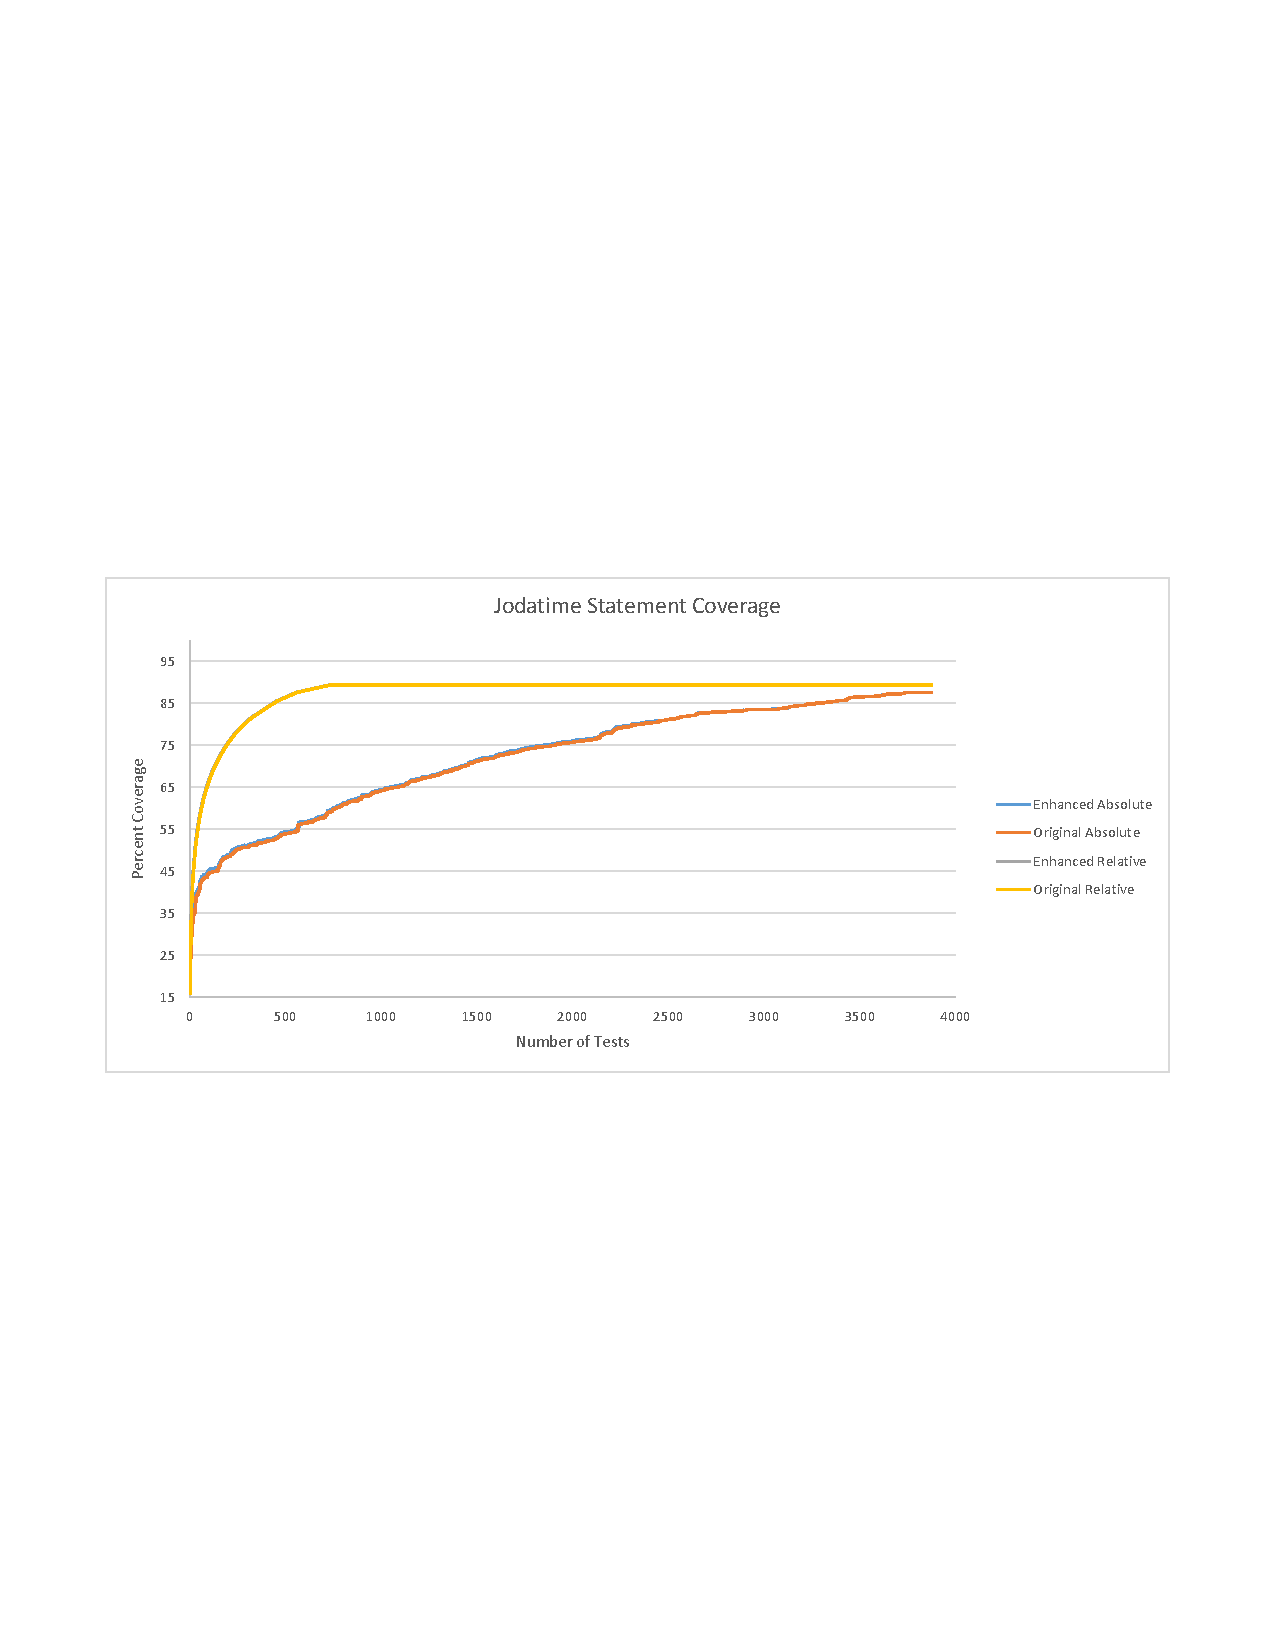
\includegraphics[scale=0.46]{jodatime-coverage-figure}
Jodatime
%\caption{replace} \label{fig:p2}
\end{minipage}
\begin{minipage}[b]{\linewidth}
\centering
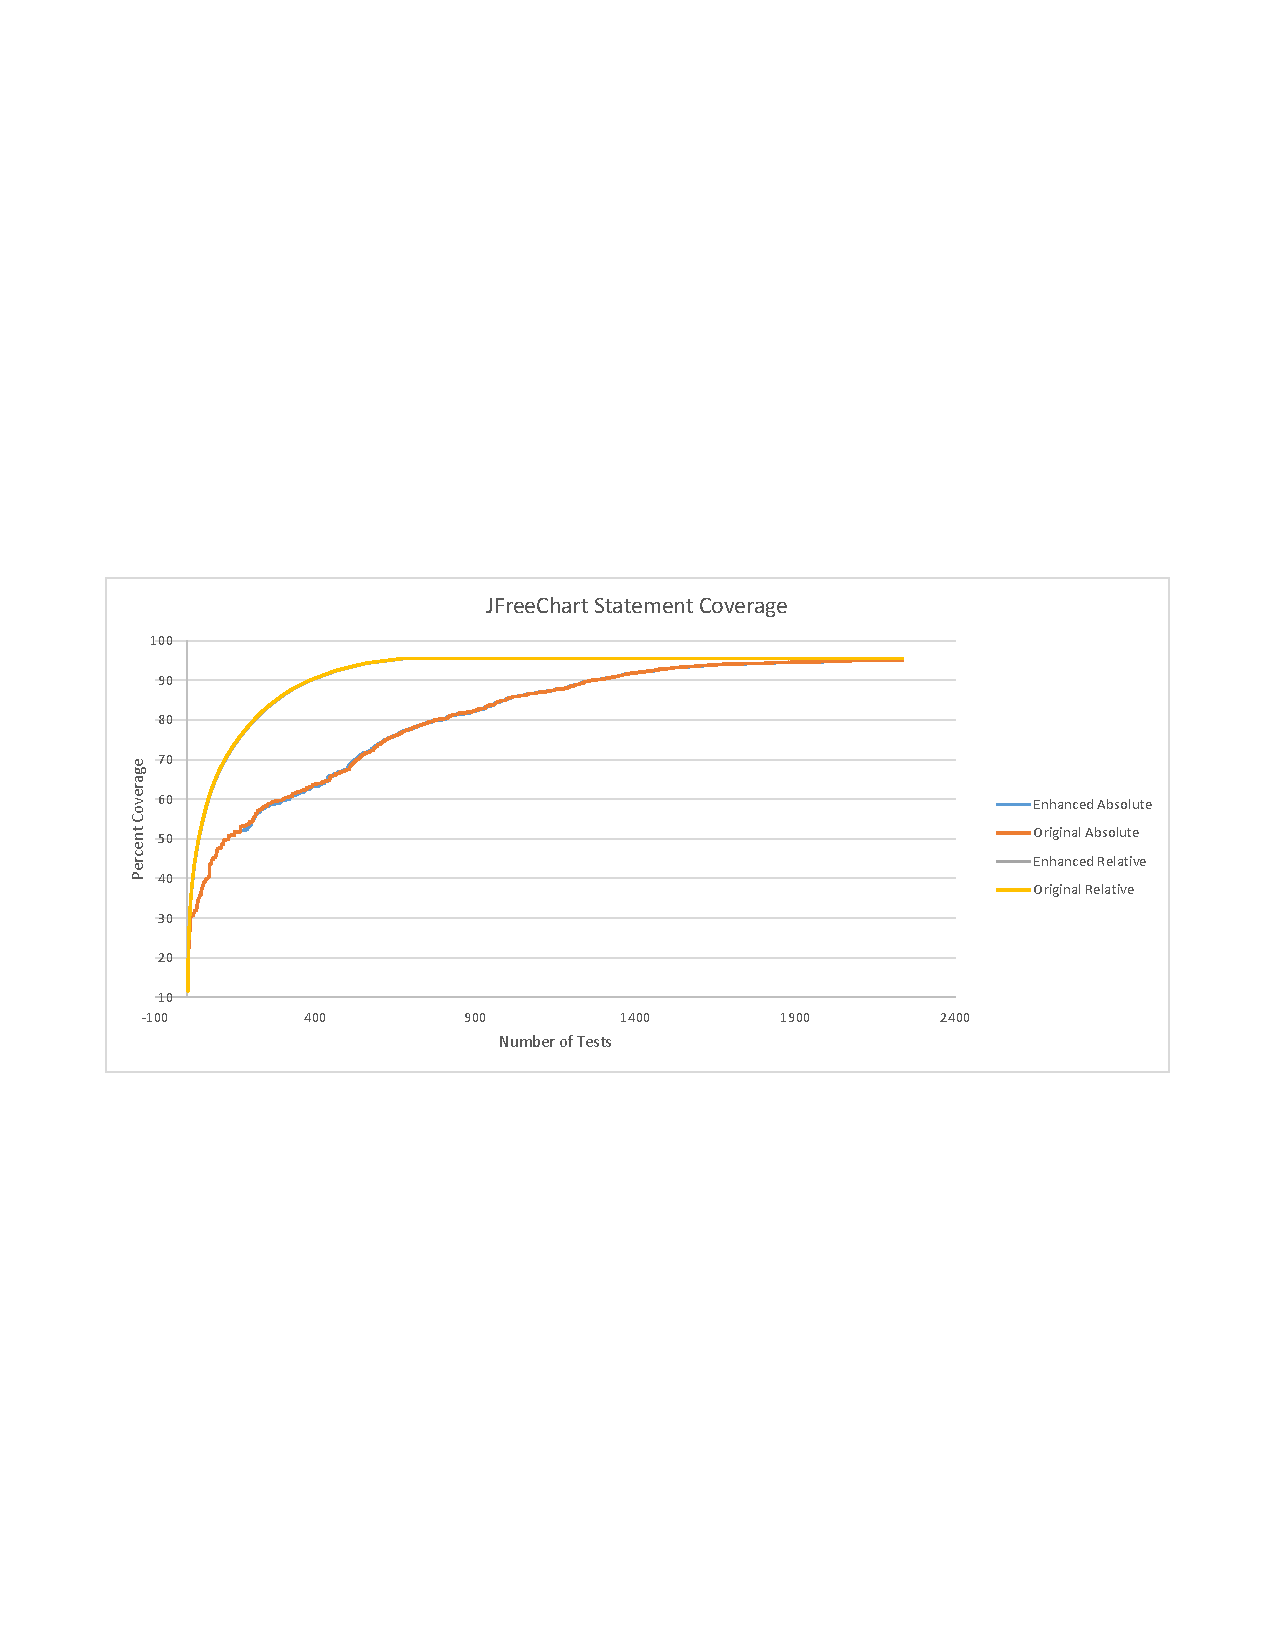
\includegraphics[scale=0.46]{jfreechart-coverage-figure}
JFreechart
%\caption{schedule} \label{fig:p3}
\end{minipage}
\begin{minipage}[b]{\linewidth}
\centering
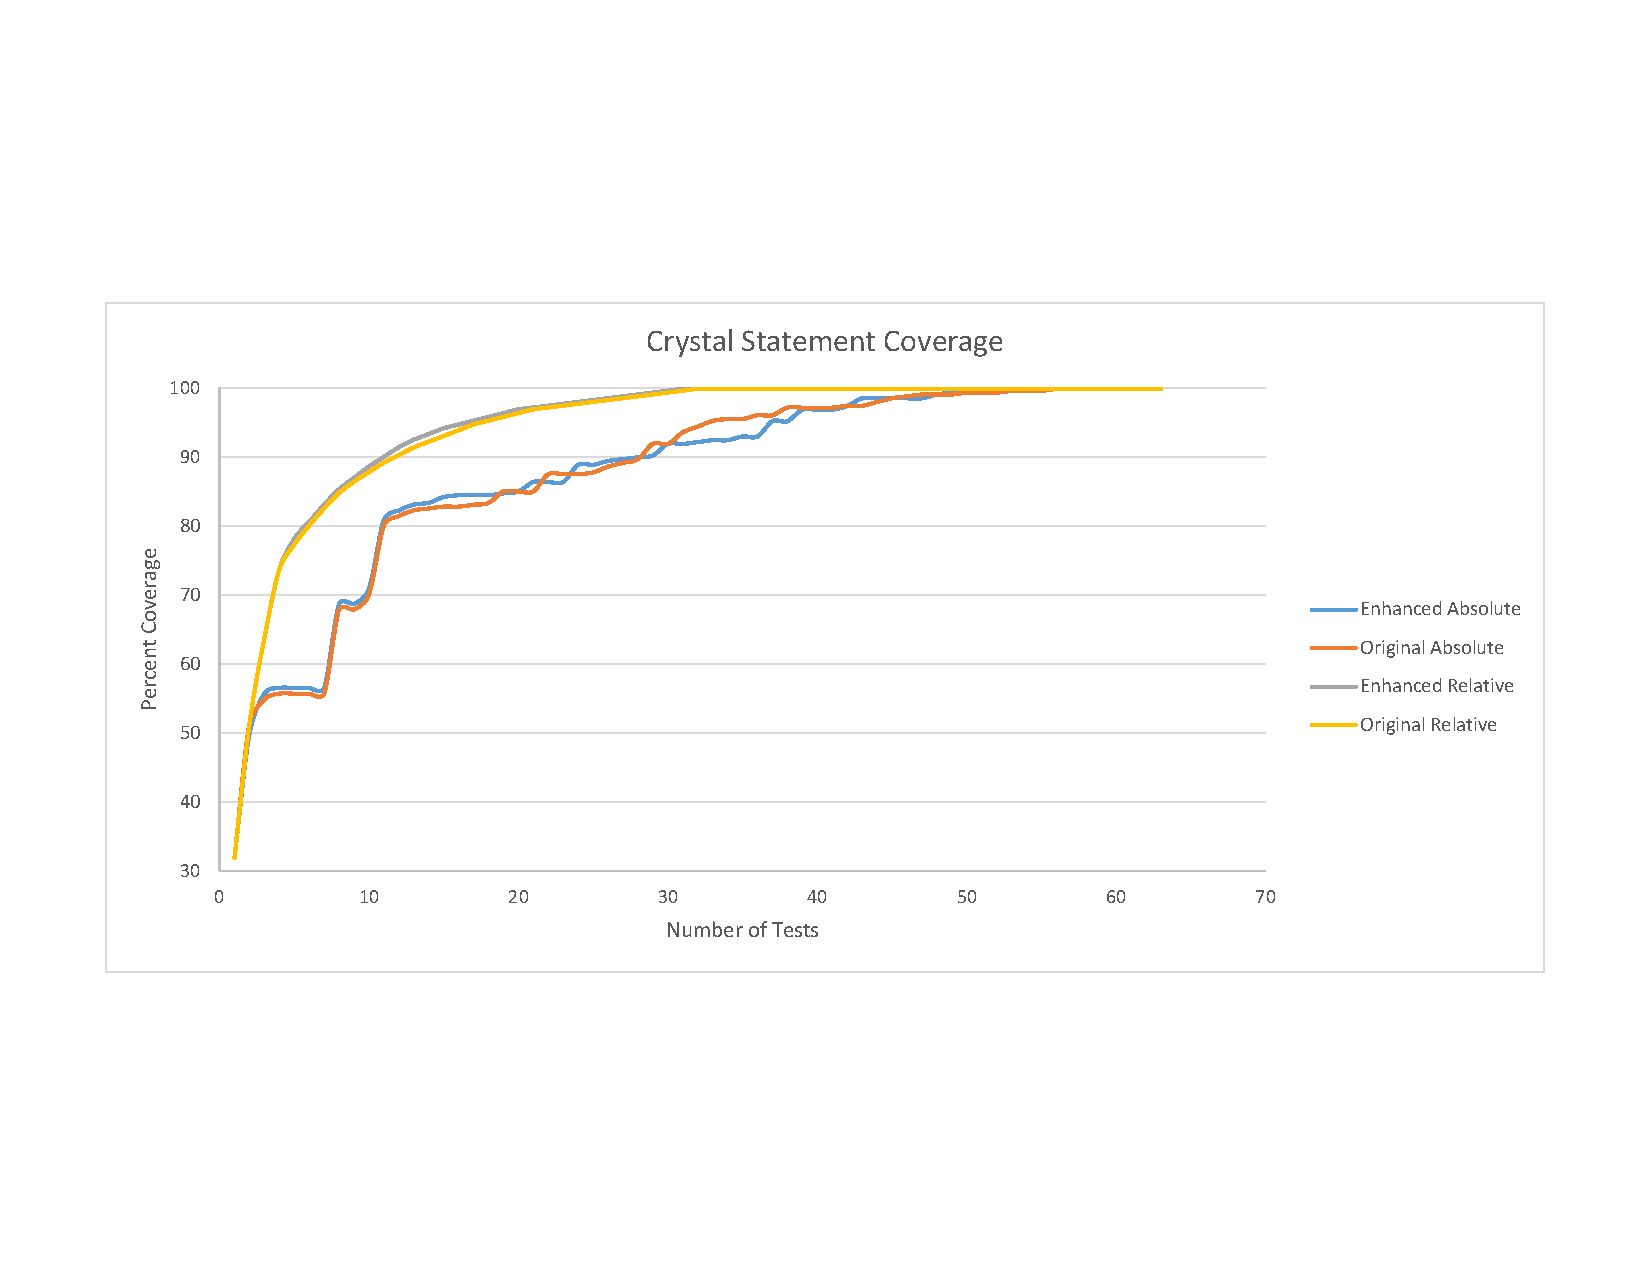
\includegraphics[scale=0.35]{crystal-coverage-figure}
{Crystal}
%\caption{tcas} \label{fig:p1}
\end{minipage}
\vspace{-6mm}
\caption{
    \label{fig:priocoverage}
Statement coverage results by each test prioritization technique on
our evaluation subject programs.
As shown in Table~\ref{tab:testprioresult}, the subject programs Synoptic
and XML-Security were omitted because none of the orders from their
nonenhanced orders revealed any dependent tests.
}
\end{figure}




\subsection{Dependence-Aware Test Prioritization}

All tests reveal the same results as being executed
in the default, unprioritized test suite in the prioritized
order produced by all enhanced, dependence-aware test
prioritization techniques. This is because when prioritizing
a test, the enhanced technique always checks whether
its depending tests have been executed before it or not. Thus,
the test dependence is preserved in the enhanced prioritized order.

We evaluate the effectiveness of the enhanced prioritized test suite
by measuring its coverage. Figure~\ref{fig:priocoverage}
shows the results. The test orders produced by the enhanced
test prioritization techniques achieves \textit{higher}
coverage \textit{faster} than the unenhanced test orders.
This was surprising because we expected a test order to achieve higher
coverage slower when we have to reorder it to preserve test dependence.
Yet the results we collected contradicted that.
Unlike the enhanced orders, dependent tests in the unenhanced orders
actually do not provide the coverage it does in the unprioritized test suite.
As an example, test $\mathit{a}$ may covers 50 statements when
executed in the unprioritized test suite. However because test
$\mathit{a}$ is dependent on test $\mathit{b}$ running before it,
if a test prioritization order does not have test $\mathit{b}$
running before test $\mathit{a}$, then test $\mathit{a}$ may only
cover a subset of the 50 statements it is expected to cover.
Common reasons for why our dependent tests achieved higher
coverage slower in our unenhanced orders was because of the
occurrences of events that disrupts the normal flow of
instructions and the different paths of execution taken for branches. 

\subsection{Dependence-Aware Test Selection}

\begin{table}
\centering
\setlength{\tabcolsep}{1.25\tabcolsep}
\begin{tabular}{|l|c|c|}
%\toprule
\hline
\textbf{Subject Program} & S1 (statement-level) & S2 (method-level)  \\
\hline
\multicolumn{3}{|l|}{}  \\
\multicolumn{3}{|l|}{\textbf{Human-written Test Suites}}  \\
\hline
\jt& 332 $\rightarrow$ 335 & 3233 $\rightarrow$ 3233 \\
XML Security& 70 $\rightarrow$ 83 & 71 $\rightarrow$ 84  \\
%\bottomrule
\hline
\textbf{Total} & 402 $\rightarrow$ 418 & 3304 $\rightarrow$ 3317 \\
\hline
%\textbf{Total}& &  & &  \\ 
%\hline
\end{tabular}
\caption{Results of evaluating the \selnum test selection techniques
in Table~\ref{tab:enhancetestsel} on four human-written unit test suites.
Each cell shows the number of selected tests.
As shown in Table~\ref{tab:testselresult}, the subject programs Crystal,
JFreeChart and Synoptic were omitted because none of the orders from their
nonenhanced orders revealed any dependent tests.
}
\label{tab:enhancedselresult}
\end{table}

All tests in the test subset selected by all test selection
techniques reveal the same result as in the default
test suite. Similar to the enhanced test prioritization
techniques, when selecting an affected test,
each enhanced test selection technique also checks whether
its depending tests have been selected and executed
before it in the selected test subset. Therefore,
the test dependence is always preserved.

We measure the size of the selected subset.  Table~\ref{tab:enhancedselresult}
shows the results. The enhanced techniques 
slightly increase the selected test subset by
less than  1\%.

\subsection{Dependence-Aware Test Parallelization}

\begin{table*}
\centering
\setlength{\tabcolsep}{1.25\tabcolsep}
\begin{tabular}{|l| l|l|l|l| l|l|l|l| l|l|l|l|}
%\toprule
\hline
\textbf{Subject Program} & \multicolumn{4}{|l|}{P1 (Original Order Parallelization)} &  \multicolumn{4}{|l|}{P2 (Random Parallelization)} & \multicolumn{4}{|l|}{P3 (Time-Minimized Parallelization)}\\
\cline{2-13}
& k=2 & k=4 & k=8 & k=16 & k=2 &k=4& k=8& k=16 & k=2 &k=4& k=8& k=16\\
\hline
\multicolumn{13}{|l|}{}  \\
\multicolumn{13}{|l|}{\textbf{Human-written Test Suites}}  \\
\hline
\jt& 3.47 & 1.97 & 1.84 & 1.80 & 2.83 & 2.61 & 1.92 & 1.80 & 2.20 & 2.11 & 1.38  & 1.79\\
XML Security& 1.45 & 1.89 & 2.48 & 5.72 & 1.56  & 2.35 & 4.02  & 4.25 & 2.56 & 2.82  & 4.38 & 6.00 \\
Crystal& 1.72  & 1.84  & 1.24  & 1.48  & 1.72 & 2.16& 1.72 & 1.04 & 2.12 & 1.34 & 1.33& 1.26\\
JFreechart&  1.33 & 1.26 & 1.15  & 1.27  & 1.44 & 1.28 & 1.30 & 1.22 & 1.46 & 1.31 & 1.31 & 1.40\\
%\bottomrule
\hline
\textbf{Average} & 1.99  & 1.74 & 1.67  & 2.57 & 1.89 & 2.10& 2.24 & 2.08 & 2.09 & 1.89 & 2.10 & 2.61\\
\hline
%\textbf{Total}& &  & &  \\ 
%\hline
\end{tabular}
\caption{
Results of evaluating the enhanced test parallelization techniques
on the subject programs. The numbers displayed in the table are
calculated from dividing the time cost to execute the enhanced
order by the time cost to execute the nonenhanced order.
As shown in Table~\ref{tab:testparresult}, the subject program Synoptic was
omitted because none of the orders from its nonenhanced orders revealed
any dependent tests.
\todo{show the slow}
}
\label{tab:enhancedparresult}
\end{table*}

By using the enhanced test parallelization techniques,
all tests scheduled on different machines reveal the
same results as being executed in the original test suite.

The major purpose of using test parallelization techniques is
to shorten the total test execution time. We measure the total
test execution time by recording the time taken by the slowest
machine. Table~\ref{tab:enhancedparresult} shows the
slowdown of each enhanced parallelization technique.
The slowdown varies across different techniques and test suites,
ranging from 1.67 to 2.61, on average. The slowdown is a result
of the increased amount of tests machines have to execute in
order to preserve test dependence. To elaborate, say test $\mathit{a}$
depends on test $\mathit{b}$ yet they were both scheduled
to be executed in different machines. In order for test $\mathit{a}$ to exhibit
the same behavior as it did in the unparallelized test suite, whichever
machine test $\mathit{a}$ is contained in will  have to have test
$\mathit{b}$ be added to it.


\subsection{Discussion}

\subsubsection{Threats to Validity}

There are several threats to the validity
of our experiments. 
%First, \dtexplain 
%only considers test dependencies arised
%from improper field access. It may not
%produce useful results for other types of
%test dependencies~\cite{}. 
First, the subject programs and the test suites
used to evaluate the enhanced testing techniques may
not be representative enough. We donot claim
our findings can be generalized to any subject
programs or test suites. Second,
when measuring the effectiveness of each enhanced
testing technique, we measure the test coverage
result, the size of the selected subset, and
the test execution time. We did not measure
Second,
\todo{evaluating on the test coverage, no
bug finding abilities yet.}

\subsubsection{Experimental Conclusions}

We have two chief findings. 
%\textbf{(1)} \dtexplain
%generates concise report to explain why
%test dependence arises, and such report
%helps developers to understand the root cause
%of test dependence.
\textbf{(1)} All enhanced downstream testing techniques
output consistent results on test suites
containing dependent tests. And \textbf{(2)}
The enhanced testing techniques have
little impact on the testing effectiveness.


\section{Related Work}
\label{sec:related}

%Denoting a group of test cases as a ``suite of test programs'' began around the
%mid-1970's~\cite[p.~217]{brown:CSUR:1974}; similar terms include
%``testcase dataset''~\cite{milleretal:ICRS:1975} and ``scenario,''
%which an IEEE Standard defines as ``groups of test cases;
%synonyms are script, set, or suite''~\cite[p.~10]{IEEE:829-1998}.

Treating test suites explicitly as \emph{mathematical sets} of tests dates at least
to Howden~\cite[p.~554]{howden:ToC:1975} and remains common in the literature.
The execution order of tests in a suite is usually not considered:
%or informally, suggesting that the potential of executing a given test
%in different contexts is immaterial to those results: 
that is, test independence is assumed. We next discuss some
existing definitions of test dependence, techniques that
assume test dependence, and tools that support specifying
test dependence.


\subsection{Test Dependence}

Definitions in the testing literature are generally clear that the
conditions under which a test is executed may affect its result. 
The
importance of context in testing has been explored in some depth in
some domains including databases~\cite{Gray:1994:QGB:191843.191886,Chays:2000:FTD:347324.348954,
kapfhammeretal:FSE:2003}, with results about test
generation, test adequacy criteria, etc., and mobile
applications~\cite{Wang:2007:AGC}.
For the database domain, Kapfhammer and Soffa formally
define independent test suites and distinguish them from
other suites that ``can capture more of an application's
interaction with a database while requiring the constant monitoring of
database state and the potentially frequent re-computations of test
adequacy''~\cite[p.~101]{kapfhammeretal:FSE:2003}.
By contrast, our definition differs from that of Kapfhammer
and Soffa by considering
test results rather than program and database states
(which may not be visible to users).
%Considering only manifest test dependences allows
%us to more easily situate this research in the empirical domain (Section~\ref{sec:formaldiscussion}).

The IEEE Standard for Software and System Test
Documentation (829-1998) \S 11.2.7, ``Intercase
Dependencies,'' says in its entirety: ``List the identifiers of
test cases that must be executed prior to this test
case. Summarize
the nature of the dependences''~\cite{IEEE:829-1998}.  The succeeding version of this
standard (829-2008) adds a single sentence: ``If
test cases are documented (in a tool or otherwise) in the order in
which they need to be executed, the Intercase Dependencies for most or
all of the cases may not be needed''~\cite{IEEE:829-2008}.


%In addition to the work by Kapfhammer and
%Soffa~\cite{kapfhammeretal:FSE:2003},
%there are a handful of categorical references that
%acknowledge that tests can
%be dependent based on context, suggesting 
%ways to document or find situations where the independence
%assumption fails to hold.  


%McGregor and Korson discuss interaction tests that
%are intended to identify ``two methods that may directly or indirectly
%cause each other to produce incorrect results'' and suggest constructing such
%interaction tests by identifying the values shared via parameter passing
%between methods
% that two or more test cases share~\cite[p~.69]{mcgregoretal:CACM:1994}.

Bergelson and Exman characterize a form of test dependence informally:
given two tests that each pass, the composite
execution of these tests may still
fail~\cite[p.~38]{bergelsonetal:EEE:2006}.  That is, if 
\suite{t_1} executed by itself passes and \suite{t_2} executed by itself passes,
executing the sequence \suite{t_1, t_2} in the same context may fail.
However, they do not provide any empirical evidence of
test dependence nor any detection algorithms.

Some practitioners acknowledge test dependence as a possible, albeit low probability, event:
\begin{quote}
Unit testing \dots  
requires that we test the unit in isolation. That is, we
want to be able to say, \emph{to a very high degree of confidence} [emphasis added], that
any actual results obtained from the execution of test cases are
purely the result of the unit under test. The introduction of
other units may color our results~\cite{unit-test-def}.
\end{quote}
They further note that other tests, as well as stubs and drivers,
may ``interfere with the straightforward
execution of one or more test cases.''


Compared with these informal definitions,
we formalize test dependence, and provide empirical evidence
to show that test dependence does arise in practice, and could
have costly repercussions.
%They give an informal definition of what it means for the execution of a
%test to influence the outcome of another test.  We define
%this precisely, and we also define manifest test dependence in terms
%of execution environments
%and test execution order rather than in terms of code use.

%Other definitions of test dependence are primarily considered
%to be \textit{syntactic} dependences between program units, for example
%methods calling other methods, and classes using other classes~\cite{bergelsonetal:EEE:2006,briandetal:SEKE:2002}. 
%\emph{Syntactic} dependence here means that a unit \code{A} cannot be
%compiled and executed without unit \code{B} being present. If we test
%such a unit \code{A} without convincing ourselves first that \code{B}
%is correct, a test failure for \code{A} is harder to interpret,
%because it could just as well indicate a fault in \code{B}.
%Zhang and Ryder extend this notion to \emph{semantic} dependences,
%which is closer to our approach~\cite{zhangetal:TR:2006}. 
%They use a notion of
%``test outcome'' to determine whether or not syntactically dependent
%classes or methods can influence each others results, and consider
%only those that can to be semantically dependent.
%They give an informal definition of what it means for the execution of a
%test to influence the outcome of another test.  We define
%this precisely, and we also define manifest test dependence in terms
%of execution environments
%and test execution order rather than in terms of code use.


\subsection{Techniques Assuming Test Independence}

The assumption of test independence lies at the heart of most,
if not all, techniques for automated regression test selection,
test case prioritization, test generation, coverage-based
fault localization, etc. 


Test prioritization seeks to reorder a test suite to detect
software defects more quickly. 
Early work in test
prioritization~\cite{Wong:1997:SER:851010.856115,Rothermel:1999:TCP:519621.853398}
laid the foundation for the most commonly used problem definition:
consider the set of all permutations of a test suite and find the best
award value for an objective function over that
set~\cite{Elbaum:2000:PTC:347324.348910}.  The most common objective
functions favor permutations where more faults in the underlying
program  are found with running fewer tests.
Test independence is often explicitly asserted as a
requirement for most test selection and prioritization work (e.g.,~\cite[p.~1500]{Rummel:2005:TPR:1066677.1067016}).
%For some test selection and prioritization work,
%test independence is even explicitly asserted as a requirement.
%For example, Rummel et al.\ states in
%A number of studies carefully evaluation various prioritization techniques
%empirically~\cite[\emph{et
%alia}]{Rothermel:1999:TCP:519621.853398,Do:2010:ETC:1907658.1908088}. 
Evaluations of selection and prioritization techniques
~\cite[\emph{et alia}]{Rothermel:1999:TCP:519621.853398,Do:2010:ETC:1907658.1908088}
are based in part on the test independence
assumption as well as the assumption that the set of faults in the underlying
program is known beforehand; the possibility that test dependence may unmask additional faults in the program is not studied.

%\begin{quote}
%A test suite contains a tuple of tests \suite{T_1 $\ldots$ T_R} that execute in a specified order.  We require that each test is
%independent so that there are no test execution ordering dependencies.  This requirement enables our prioritization algorithm to
%re-order the tests in any sequence that maximizes the suite's
%ability to isolate defects.  The assumption of test dependence
%is acceptable because the JUnit test execution framework
%provides \code{setUp} and \code{tearDown} methods that execute before
%and after a test case and can be used to clear application
%state.
%\end{quote}

Most automated test generation
techniques~\cite{PachecoLET2007, Wang:2007:AGC,
ZhangSBE2011} do not take test dependence
into consideration. As shown in our experiments (Section~\ref{sec:evaluation}),
a large number of tests generated by Randoop are dependent.
We speculate that these dependences arise because automated
test generation techniques generally create new tests
based on the program state after executing the previous test,
for the sake of test diversity and efficiency. 
To the best of our knowledge, only JCrasher~\cite{Csallner:2004}
provides a mode to clear the environment changes caused
by a previous test. Such functionality helps eliminate
potential test dependence, but may make generated
tests less behaviorally-diverse --- as they cannot be constructed
on top of previous tests. Exploring how to
incorporate test dependence into the design of automated
test generator is our future work.

Coverage-based fault localization techniques~\cite{Jones:2002:VTI}
often treat a test suite as a collection of test cases
whose result is \textit{independent} of the order of their
execution. They can also be impacted by test dependence.
In a recent evaluation of several coverage-based fault locators,
 Steimann et al.\ found fault locators' accuracy has been significantly
 affected by tests failed due to the violation of the test
 independence assumption~\cite{Steimann:2013}. 
 %For example, if a test depends on a static field whose value is set by
 %previous test cases. 
 Compared to our work, Steimann et al.'s
 work focuses on identifying possible threats to validity
 in evaluating coverage-based fault localization, and does
 not present any formalism, study, or detection algorithms
 for dependent tests.


%define a test suite as a
%collection of test cases whose result is \textit{independent}
%of the order of their execution~\cite{Steimann:2013}.

As shown in Sections~\ref{sec:study} and~\ref{sec:evaluation},
the test independence assumption often does not hold for either
human-written or automatically-generated tests. Thus, techniques
that rely on this assumption may need to be reformulated.

\subsection{Tools Supporting Test Dependence}
\label{sec:supporting}

Testing frameworks provide mechanisms
for developers to define the context for tests.
JUnit, for example, provides means to
automatically execute setup and clean-up tasks
(\code{setUp()} and \code{tearDown()} in JUnit
3.x, and methods annotated with \code{@Before} and \code{@After} in
JUnit 4.x). Ensuring that these mechanisms are used properly, however, is
beyond the scope of any framework, although the latest release of JUnit
(version 4.11)
supports executing tests in lexicographic order by test method name~\cite{junitordering}.


Only a few tools explicitly consider test dependence, by
allowing developers to annotate dependent tests and
provide supporting mechanisms to ensure that the test execution framework
respects those annotations.  DepUnit~\cite{depunit}
allows developers to define soft and hard dependences. Soft dependences control
test ordering, while hard dependences in addition control whether specific tests are
run at all.  TestNG~\cite{testng} 
allows dependence annotations and supports a variety of execution policies
that respect these dependences
such as sequential execution
in a single thread, execution of a single test class per thread, etc.\
What distinguishes our work from these approaches is that, while they allow dependences
to be made explicit and respected during execution, they do not help developers
\emph{identify} dependences.  A tool that finds dependences
(Section~\ref{sec:impl}) could co-exist
with such frameworks by generating annotations for them.

Our previous work~\cite{DBLP:conf/sigsoft/MusluSW11} proposed
an algorithm to find bugs by executing each unit
test in isolation. With a different focus,
this work investigates the validity of the test independence assumption
rather than finding new bugs,
and presents four new results.
Further, as indicated by our study and experiments, most dependent
tests reveal weakness in the test code rather than bugs in the program. Thus,
using test dependence may not achieve a high return in finding bugs.

%  LocalWords:  Howden Kapfhammer Soffa dependences Intercase Bergelson
%  LocalWords:  Exman JCrasher Steimann setUp tearDown DepUnit TestNG


\section{Conclusion and Future Work}

Test independence is broadly assumed but rarely addressed, and
the impact of test dependence has largely been ignored in previous research
on software testing. This paper describes
one of the first empirical studies on real-world test suites to
understand the impact of test dependence. The experimental
results show that test dependence \textit{does} affect the results
of many popular test prioritization, test selection, and test
parallelization techniques. To cope with the impact of test
dependence, this paper proposes a family of techniques
to enhance existing testing techniques, making them respect test dependence
and produce consistent testing results.


Our results are suggestive to practitioners and researchers.
Both can learn that the impact of test dependence 
should not be ignored any longer. Researchers are posed important
but challenging problems in design new testing techniques,
such as how to adapt testing methodologies to account for
dependent tests how to detect and correct all dependent tests.

Our future work should focus on the following directions:

\vspace{1mm}

\noindent \textbf{{Investigating impact of dependent tests
on other downstream testing techniques.}}
We have shown that dependent tests can compromise the application of
\prionum test prioritization, \selnum test selection,
and \parnum test parallelization techniques.
%assumption is not true. However,
We plan to conduct comprehensive empirical studies to
measure the impact of dependent tests on other
downstream techniques, such as mutation testing~\cite{},
test factoring~\cite{}, and experimental
debugging techniques~\cite{}.
We are also interested in developing techniques that can enhance these
testing techniques to respect test dependence.



\vspace{1mm}

\noindent \textbf{{Eliminating dependent tests.}}
As reflected in our previous study~\cite{},
the practice of eliminating dependent tests
remains mostly manual and ad hoc --- software developers
usually manually hardcode test
execution orders in a configuration file or
simply merge or remove tests.
A more flexible and robust methodology for
dependent test elimination should be developed.
%While our technique proposed in Section~\ref{}
%provides a first step in understanding the root cause
%of test dependence, the question
%of automatically removing dependent tests
%still remains open.
This question also applies to automated test generators,
and some work has been developed to alleviate
this problem~\cite{vmvm, RobinsonEPAL2011,fraseretal:ISSTA:2011}.




\begin{comment}

The topic of test dependence has been largely ignored in previous research on software testing, particularly its effects on testing techniques such as test prioritization. We believe we are the first to study the impact test dependence has on test prioritization through the application of test prioritization techniques on real-world programs. Other studies of applying test prioritization techniques to real-world programs include one from August 2000~\cite{} and another from October 2001~\cite{}. Although we concluded that the impact of dependent tests on test prioritization is minimal, we showed that test dependence does indeed affect the execution results of test prioritization techniques. We were able to show this by designing and implementing five test prioritization techniques and applying them to five real-world programs. Lastly, we described impending features to our set of existing tools that when generating test prioritization execution orders will take into account which tests depend on one another. 

Our future work should focus on the following directions:
\begin{itemize}
\item Understand the impact test dependence may have on other testing techniques. Dependent tests can compromise the application of testing techniques such as test generation, selection, prioritization, and parallelization, since most current testing techniques just assume independence and make no statement about what happens when this assumption is not true [1]. In this paper we have addressed how test dependence affect five test prioritization techniques. Our future work will consist of studying the effects of test dependence on other test prioritization techniques particularly branch coverage and other test techniques such as test selection. 
\item Preventing dependent tests. By preventing developers from writing dependent tests, we can eliminate the impact dependent tests will have on testing techniques. Developers should be encouraged to write tests ''defensively'' by specifying necessary test execution pre-conditions and using less (or properly mocking) global variables or shared resources. There is already some work aiming at automating this process to prevent the potential for dependences by refactoring programs to use less global states [9].
\end{itemize}
\end{comment}


%\vspace{2mm}

%\balance

\bibliographystyle{abbrv}
%\small{
%\bibliography{confdiagnoser}
\bibliography{references}
%}
\end{document}

%  LocalWords:  '12 Multithreaded Hao szhang hlv mernst Manu Sridharan ABB
%  LocalWords:  CCF
